\documentclass[]{AVSSimReportMemo}
\usepackage{AVS}


\newcommand{\ModuleName}{hillPoint}
\newcommand{\subject}{Guidance Module for Hill Frame Pointing}
\newcommand{\status}{Initial Version}
\newcommand{\preparer}{M. Cols}
\newcommand{\summary}{Generate the attitude reference to perform a constant pointing towards a Hill frame orbit axis}


\begin{document}

\makeCover


%
%	enter the revision documentation here
%	to add more lines, copy the table entry and the \hline, and paste after the current entry.
%
\pagestyle{empty}
{\renewcommand{\arraystretch}{2}
\noindent
\begin{longtable}{|p{0.5in}|p{4.5in}|p{1.14in}|}
\hline
{\bfseries Rev}: & {\bfseries Change Description} & {\bfseries By} \\
\hline
Draft & initial copy & M. Cols \\
\hline

\end{longtable}
}

\newpage
\setcounter{page}{1}
\pagestyle{fancy}

\tableofcontents
~\\ \hrule ~\\

\begin{figure}[htb]
	\centerline{
	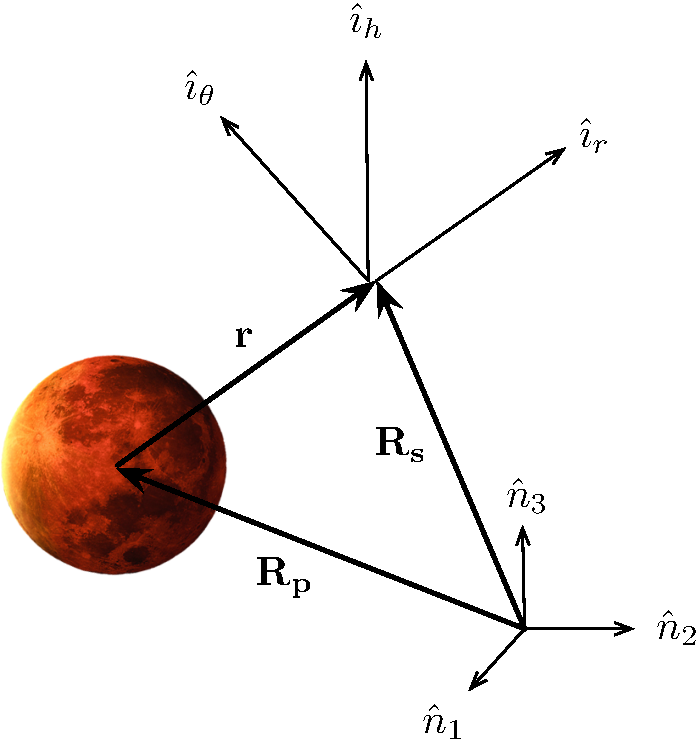
\includegraphics[width=5cm]{Figures/hillPoint}
	}
	\caption{Illustration of the Hill orbit frame $\mathcal{H}:\{ \hat{\bm\imath}_{r}, \hat{\bm\imath}_{\theta}, \hat{\bm\imath}_{h} \}$, and the inertial frame $\mathcal{N}:\{ \hat{\bm n}_{1}, \hat{\bm n}_{2}, \hat{\bm n}_{3} \}$.}
	\label{fig:Fig1}
\end{figure}

\section{Reference Frame Definition}
The Hill reference frame takes the spacecraft's orbital plane as the principal one and has origin in the center of the main celestial body. It is defined by the right-handed set of axes $\mathcal{H}:\{ \hat{\bm\imath}_{r}, \hat{\bm\imath}_{\theta}, \hat{\bm\imath}_{h} \}$, where\par
$\hat {\bm\imath}_{r}$  points radially outward in the direction that connects the center of the planet with the spacecraft. \par
$\hat {\bm\imath}_{h}$ is defined normal to the orbital plane in the direction of the angular momentum. \par
$\hat {\bm\imath}_{\theta}$ completes the right-handed triode.

\section{Introduction}
In this module, a general axis is to be aligned with a principal Hill-frame axis and stay pointing fixedly on it. Note that the presented technique does not require the Hill orbit frame $\mathcal{H}$ to coincide with the inertial frame $\mathcal{N}:\{ \hat{\bm n}_{1}, \hat{\bm n}_{2}, \hat{\bm n}_{3} \}$. Figure 1 illustrates the general situation in which $\bm{R}_{s}$ is the position vector of the spacecraft with respect to the inertial frame and $\bm{R_{p}}$ is the position vector of the orbited celestial body with respect to the inertial frame as well.
The relative position of the spacecraft with respect to the planet is obtained by simple substraction:
\begin{equation}
	\label{eq:r}
	\bm r = \bm R_{s} -  \bm R_{p}
\end{equation}
The same methodolgy is applied to compute the relative velocity vector:
\begin{equation}
	\label{eq:v}
	\bm v = \bm v_{s} -  \bm v_{p}
\end{equation}
Having $\bm r$ and $\bm v$, the Hill frame orientation is completely defined:
\begin{subequations}
	\begin{equation}
	\hat{\bm\imath}_{r} = \frac{\bm r}{r} 
	\end{equation}
	\begin{equation}
	\hat{\bm\imath}_{h} = \frac{\bm{r}\times{\bm{v}}}{r · v}
	\end{equation}
	\begin{equation}
	\hat{\bm\imath}_{\theta} = \hat{\bm\imath}_{h} \times \hat{\bm\imath}_{r}
	\end{equation}
\end{subequations}


\section{Angular Velocity Descriptions}
Let $\mathcal{R}_{0}$ reference the Hill orbit frame. The orbit frame angular rate and acceleration vectors are given by 
\begin{equation}
	\label{eq:omega_R0}
	\bm\omega_{R_{0}/N} = \dot f \hat{\bm\imath}_{h} 
\end{equation}
\begin{equation}
	\label{eq:domega_R0}
	\dot{\bm\omega}_{R_{0}/N} = \ddot f \hat{\bm\imath}_{h} 
\end{equation}
where $f$ is the true anomaly, whose variation is determined through the general standard astrodynamics relations:
\begin{align}
  \dot f &= \frac{h}{r^{2}}
  \\
  \ddot f &= - 2 \frac{\bm v \cdot \hat{\bm\imath}_{r}}{r} \dot f
\end{align}
Let the sought general reference frame be $\mathcal{R}$. The attitude tracking control requires the angular rate $\bm\omega_{R/N}$ and acceleration $\dot{\bm\omega}_{R/N}$. 
Since the pointing towards the orbit axis is constant, the desired reference $\mathcal{R}$ does not move relative to $\mathcal{R}_{0}$. Thus, the angular velocity of the reference frame happens to be
\begin{equation}
	\label{eq:omega_R}
	\bm\omega_{R/N} = \bm\omega_{R/R_{0}} - \bm\omega_{R_{0}/N} = \dot{f} \hat{\bm\imath}_{h}
\end{equation}
It is straightforward to compute the acceleration vector of the reference frame
\begin{equation}
	\label{eq:domega_R}
	\dot\omega_{R/N} = \ddot{f} \hat{\bm\imath}_{h}
\end{equation}

\bibliographystyle{unsrt}
\bibliography{references}

\end{document}
